\documentclass[twoside]{book}

% Packages required by doxygen
\usepackage{calc}
\usepackage{doxygen}
\usepackage{graphicx}
\usepackage[utf8]{inputenc}
\usepackage{makeidx}
\usepackage{multicol}
\usepackage{multirow}
\usepackage{textcomp}
\usepackage[table]{xcolor}

% Font selection
\usepackage[T1]{fontenc}
\usepackage{mathptmx}
\usepackage[scaled=.90]{helvet}
\usepackage{courier}
\usepackage{amssymb}
\usepackage{sectsty}
\renewcommand{\familydefault}{\sfdefault}
\allsectionsfont{%
  \fontseries{bc}\selectfont%
  \color{darkgray}%
}
\renewcommand{\DoxyLabelFont}{%
  \fontseries{bc}\selectfont%
  \color{darkgray}%
}

% Page & text layout
\usepackage{geometry}
\geometry{%
  a4paper,%
  top=2.5cm,%
  bottom=2.5cm,%
  left=2.5cm,%
  right=2.5cm%
}
\tolerance=750
\hfuzz=15pt
\hbadness=750
\setlength{\emergencystretch}{15pt}
\setlength{\parindent}{0cm}
\setlength{\parskip}{0.2cm}
\makeatletter
\renewcommand{\paragraph}{%
  \@startsection{paragraph}{4}{0ex}{-1.0ex}{1.0ex}{%
    \normalfont\normalsize\bfseries\SS@parafont%
  }%
}
\renewcommand{\subparagraph}{%
  \@startsection{subparagraph}{5}{0ex}{-1.0ex}{1.0ex}{%
    \normalfont\normalsize\bfseries\SS@subparafont%
  }%
}
\makeatother

% Headers & footers
\usepackage{fancyhdr}
\pagestyle{fancyplain}
\fancyhead[LE]{\fancyplain{}{\bfseries\thepage}}
\fancyhead[CE]{\fancyplain{}{}}
\fancyhead[RE]{\fancyplain{}{\bfseries\leftmark}}
\fancyhead[LO]{\fancyplain{}{\bfseries\rightmark}}
\fancyhead[CO]{\fancyplain{}{}}
\fancyhead[RO]{\fancyplain{}{\bfseries\thepage}}
\fancyfoot[LE]{\fancyplain{}{}}
\fancyfoot[CE]{\fancyplain{}{}}
\fancyfoot[RE]{\fancyplain{}{\bfseries\scriptsize Generated on Sat Jan 20 2018 07\-:59\-:02 for My Project by Doxygen }}
\fancyfoot[LO]{\fancyplain{}{\bfseries\scriptsize Generated on Sat Jan 20 2018 07\-:59\-:02 for My Project by Doxygen }}
\fancyfoot[CO]{\fancyplain{}{}}
\fancyfoot[RO]{\fancyplain{}{}}
\renewcommand{\footrulewidth}{0.4pt}
\renewcommand{\chaptermark}[1]{%
  \markboth{#1}{}%
}
\renewcommand{\sectionmark}[1]{%
  \markright{\thesection\ #1}%
}

% Indices & bibliography
\usepackage{natbib}
\usepackage[titles]{tocloft}
\setcounter{tocdepth}{3}
\setcounter{secnumdepth}{5}
\makeindex

% Hyperlinks (required, but should be loaded last)
\usepackage{ifpdf}
\ifpdf
  \usepackage[pdftex,pagebackref=true]{hyperref}
\else
  \usepackage[ps2pdf,pagebackref=true]{hyperref}
\fi
\hypersetup{%
  colorlinks=true,%
  linkcolor=blue,%
  citecolor=blue,%
  unicode%
}

% Custom commands
\newcommand{\clearemptydoublepage}{%
  \newpage{\pagestyle{empty}\cleardoublepage}%
}


%===== C O N T E N T S =====

\begin{document}

% Titlepage & ToC
\hypersetup{pageanchor=false}
\pagenumbering{roman}
\begin{titlepage}
\vspace*{7cm}
\begin{center}%
{\Large My Project }\\
\vspace*{1cm}
{\large Generated by Doxygen 1.8.6}\\
\vspace*{0.5cm}
{\small Sat Jan 20 2018 07:59:02}\\
\end{center}
\end{titlepage}
\clearemptydoublepage
\tableofcontents
\clearemptydoublepage
\pagenumbering{arabic}
\hypersetup{pageanchor=true}

%--- Begin generated contents ---
\chapter{R\-E\-A\-D\-M\-E}
\label{md_README}
\hypertarget{md_README}{}
Proiect Retele 
\chapter{Hierarchical Index}
\section{Class Hierarchy}
This inheritance list is sorted roughly, but not completely, alphabetically\-:\begin{DoxyCompactList}
\item \contentsline{section}{Crypto}{\pageref{classCrypto}}{}
\item \contentsline{section}{Data\-Base}{\pageref{classDataBase}}{}
\item \contentsline{section}{Parser}{\pageref{classParser}}{}
\item \contentsline{section}{Request}{\pageref{classRequest}}{}
\item \contentsline{section}{Response}{\pageref{classResponse}}{}
\item \contentsline{section}{th\-Data}{\pageref{structthData}}{}
\item \contentsline{section}{Token}{\pageref{classToken}}{}
\begin{DoxyCompactList}
\item \contentsline{section}{Operand}{\pageref{classOperand}}{}
\item \contentsline{section}{Operator}{\pageref{classOperator}}{}
\end{DoxyCompactList}
\item \contentsline{section}{Tree}{\pageref{classTree}}{}
\end{DoxyCompactList}

\chapter{Class Index}
\section{Class List}
Here are the classes, structs, unions and interfaces with brief descriptions\-:\begin{DoxyCompactList}
\item\contentsline{section}{\hyperlink{classCrypto}{Crypto} }{\pageref{classCrypto}}{}
\item\contentsline{section}{\hyperlink{classDataBase}{Data\-Base} }{\pageref{classDataBase}}{}
\item\contentsline{section}{\hyperlink{classOperand}{Operand} }{\pageref{classOperand}}{}
\item\contentsline{section}{\hyperlink{classOperator}{Operator} }{\pageref{classOperator}}{}
\item\contentsline{section}{\hyperlink{classParser}{Parser} }{\pageref{classParser}}{}
\item\contentsline{section}{\hyperlink{classRequest}{Request} }{\pageref{classRequest}}{}
\item\contentsline{section}{\hyperlink{classResponse}{Response} }{\pageref{classResponse}}{}
\item\contentsline{section}{\hyperlink{structthData}{th\-Data} }{\pageref{structthData}}{}
\item\contentsline{section}{\hyperlink{classToken}{Token} }{\pageref{classToken}}{}
\item\contentsline{section}{\hyperlink{classTree}{Tree} }{\pageref{classTree}}{}
\end{DoxyCompactList}

\chapter{Class Documentation}
\hypertarget{classCrypto}{\section{Crypto Class Reference}
\label{classCrypto}\index{Crypto@{Crypto}}
}
\subsection*{Static Public Member Functions}
\begin{DoxyCompactItemize}
\item 
\hypertarget{classCrypto_a1415bcac3387c1142656a4d4a33c5ea8}{static std\-::string {\bfseries sha256} (const std\-::string \&str)}\label{classCrypto_a1415bcac3387c1142656a4d4a33c5ea8}

\end{DoxyCompactItemize}


The documentation for this class was generated from the following files\-:\begin{DoxyCompactItemize}
\item 
Crypto.\-h\item 
Crypto.\-cpp\end{DoxyCompactItemize}

\hypertarget{classDataBase}{\section{Data\-Base Class Reference}
\label{classDataBase}\index{Data\-Base@{Data\-Base}}
}
\subsection*{Public Member Functions}
\begin{DoxyCompactItemize}
\item 
\hypertarget{classDataBase_a131e945676ae209fad9dcca64c2fcdef}{{\bfseries Data\-Base} (const std\-::string \&name)}\label{classDataBase_a131e945676ae209fad9dcca64c2fcdef}

\item 
\hypertarget{classDataBase_a6b53d823fd87e87c969e4cc1cb56eab9}{bool {\bfseries Prepare} (const std\-::string \&name)}\label{classDataBase_a6b53d823fd87e87c969e4cc1cb56eab9}

\item 
\hypertarget{classDataBase_ab2f507e2443638ca49a4c65612cf61bc}{bool {\bfseries Execute} (const std\-::string \&query)}\label{classDataBase_ab2f507e2443638ca49a4c65612cf61bc}

\item 
\hypertarget{classDataBase_a9d8dd3558ebe6723b0d6923f89949428}{bool {\bfseries Add\-Account} (std\-::string username, std\-::string password, bool admin)}\label{classDataBase_a9d8dd3558ebe6723b0d6923f89949428}

\item 
\hypertarget{classDataBase_a15cb9fb7099c197f25632681b49a094c}{bool {\bfseries Check\-Account} (std\-::string username)}\label{classDataBase_a15cb9fb7099c197f25632681b49a094c}

\item 
\hypertarget{classDataBase_abbffc7ed377bc7ade41ed7230e002eb9}{bool {\bfseries Check\-Account} (std\-::string username, std\-::string password)}\label{classDataBase_abbffc7ed377bc7ade41ed7230e002eb9}

\end{DoxyCompactItemize}


The documentation for this class was generated from the following files\-:\begin{DoxyCompactItemize}
\item 
Data\-Base.\-h\item 
Data\-Base.\-cpp\end{DoxyCompactItemize}

\hypertarget{classOperand}{\section{Operand Class Reference}
\label{classOperand}\index{Operand@{Operand}}
}
Inheritance diagram for Operand\-:\begin{figure}[H]
\begin{center}
\leavevmode
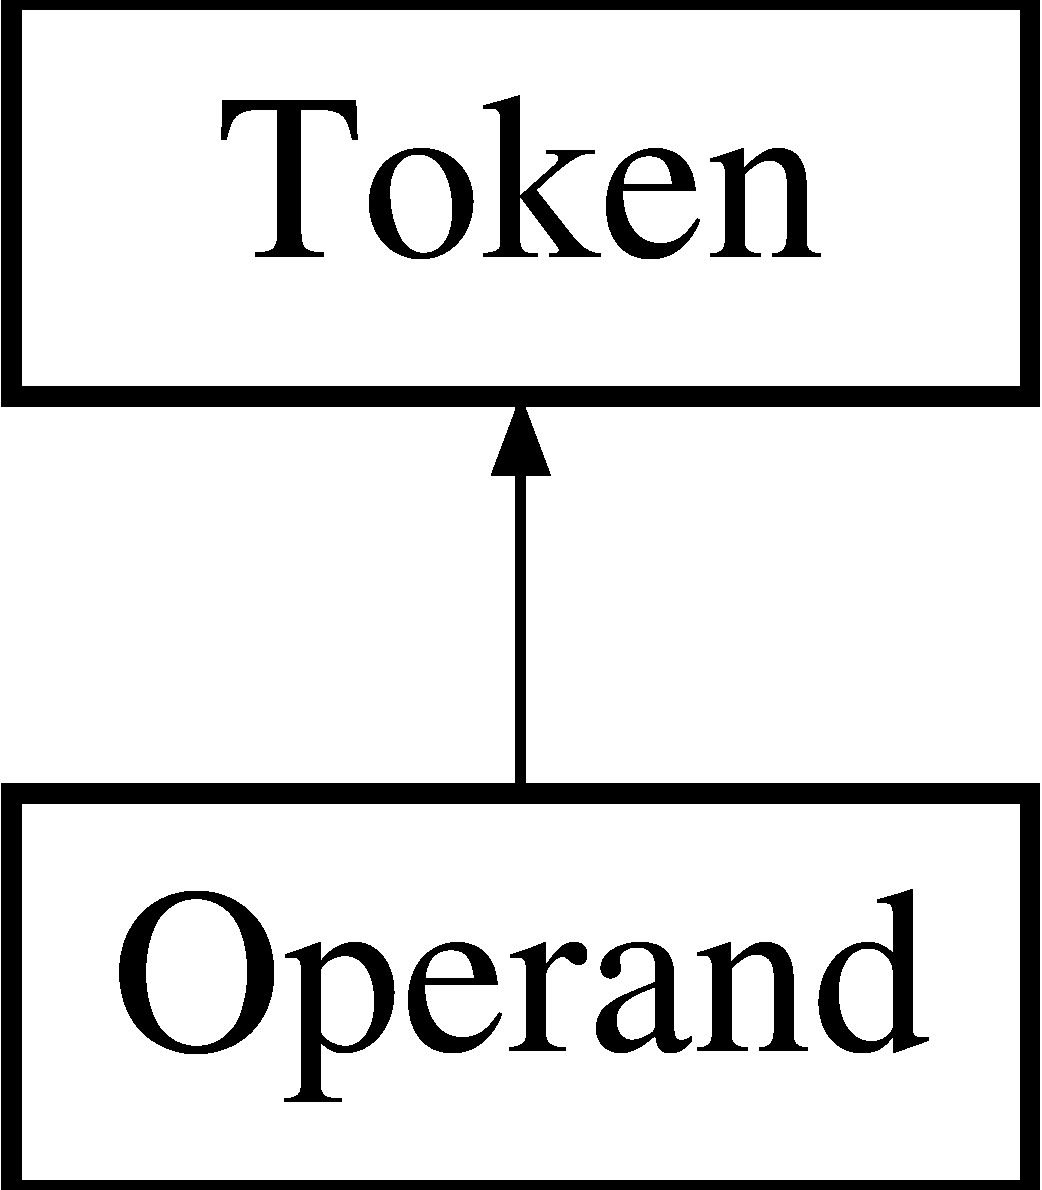
\includegraphics[height=2.000000cm]{classOperand}
\end{center}
\end{figure}
\subsection*{Public Member Functions}
\begin{DoxyCompactItemize}
\item 
\hypertarget{classOperand_a98476572f3aad95c3c5c95c25acdfeda}{{\bfseries Operand} (string com, int pr=0)}\label{classOperand_a98476572f3aad95c3c5c95c25acdfeda}

\item 
\hypertarget{classOperand_a5893a086c18e7d69ca78ae42380302c7}{string {\bfseries get\-Type} ()}\label{classOperand_a5893a086c18e7d69ca78ae42380302c7}

\end{DoxyCompactItemize}
\subsection*{Additional Inherited Members}


The documentation for this class was generated from the following file\-:\begin{DoxyCompactItemize}
\item 
operand.\-h\end{DoxyCompactItemize}

\hypertarget{classOperator}{\section{Operator Class Reference}
\label{classOperator}\index{Operator@{Operator}}
}
Inheritance diagram for Operator\-:\begin{figure}[H]
\begin{center}
\leavevmode
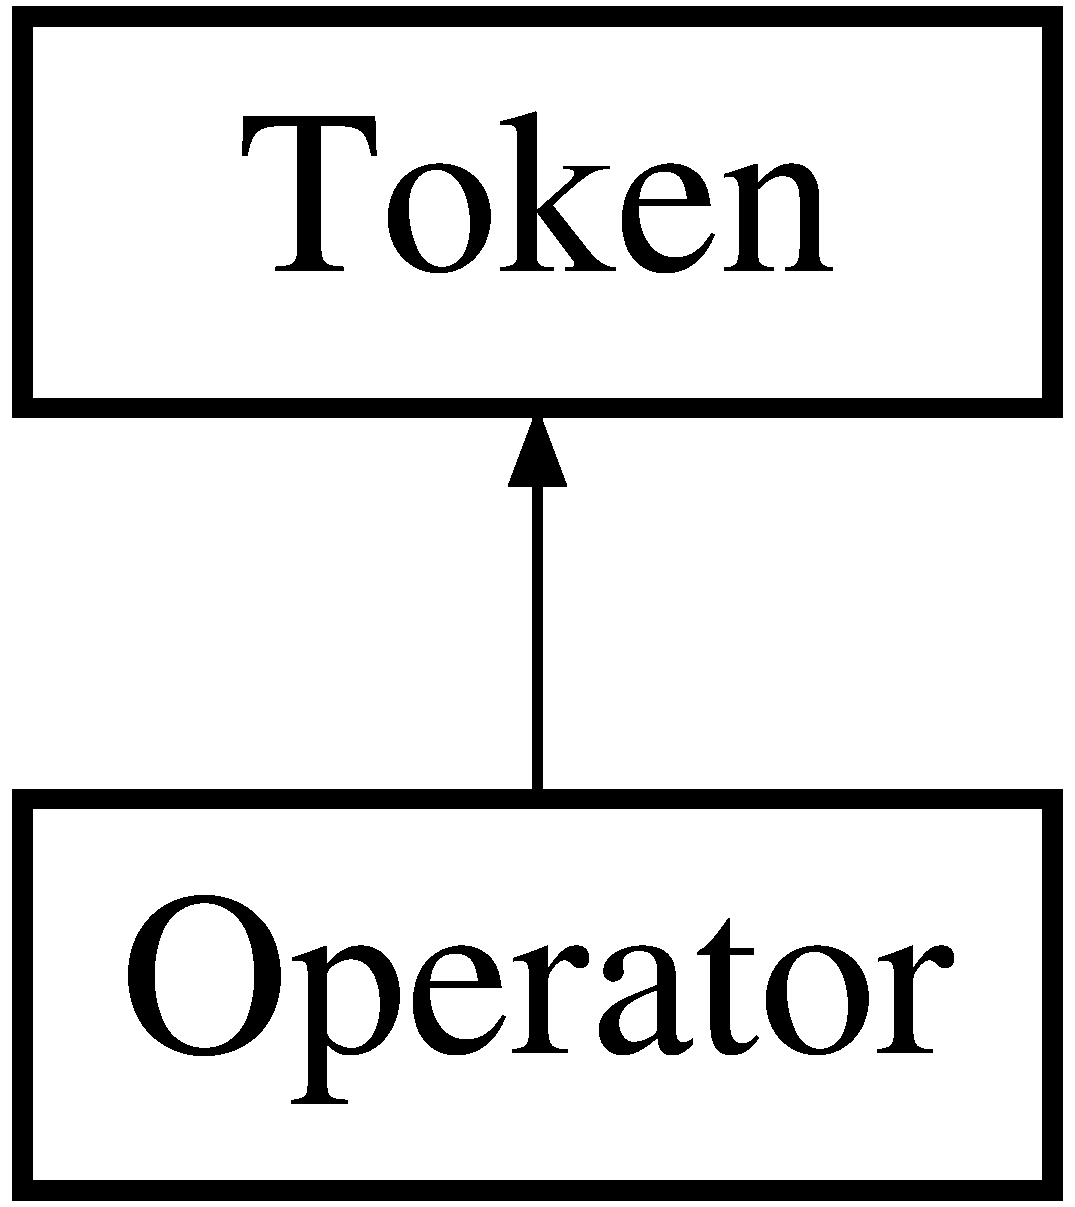
\includegraphics[height=2.000000cm]{classOperator}
\end{center}
\end{figure}
\subsection*{Public Member Functions}
\begin{DoxyCompactItemize}
\item 
\hypertarget{classOperator_a9997ab589491e1f9f6a16acebb684f32}{{\bfseries Operator} (string com, int pr=0)}\label{classOperator_a9997ab589491e1f9f6a16acebb684f32}

\item 
\hypertarget{classOperator_a53fad716ad508398daeedbbdb83ab56c}{string {\bfseries get\-Type} ()}\label{classOperator_a53fad716ad508398daeedbbdb83ab56c}

\end{DoxyCompactItemize}
\subsection*{Additional Inherited Members}


The documentation for this class was generated from the following file\-:\begin{DoxyCompactItemize}
\item 
operator.\-h\end{DoxyCompactItemize}

\hypertarget{classParser}{\section{Parser Class Reference}
\label{classParser}\index{Parser@{Parser}}
}
\subsection*{Static Public Member Functions}
\begin{DoxyCompactItemize}
\item 
\hypertarget{classParser_a1622dd8a55a1c87346f8bae8841872ff}{static void {\bfseries Parse} (const string \&input, S\-S\-L $\ast$ssl)}\label{classParser_a1622dd8a55a1c87346f8bae8841872ff}

\item 
\hypertarget{classParser_a98223ac81cb65d86b901a9218e25bf57}{static string {\bfseries Trim\-Left} (string input)}\label{classParser_a98223ac81cb65d86b901a9218e25bf57}

\item 
\hypertarget{classParser_a2252f0fb8a66f55c124e6c6b2ca3f4bb}{static string {\bfseries Trim\-Right} (string input)}\label{classParser_a2252f0fb8a66f55c124e6c6b2ca3f4bb}

\item 
\hypertarget{classParser_a91a0ce28c8cc4f6fb5f6c24998758c95}{static string {\bfseries Trim} (string input)}\label{classParser_a91a0ce28c8cc4f6fb5f6c24998758c95}

\item 
\hypertarget{classParser_a85d99169d8498e1a9dcfd12331dac704}{static queue$<$ \hyperlink{classToken}{Token} $>$ {\bfseries Parse\-Prep} (const char $\ast$input)}\label{classParser_a85d99169d8498e1a9dcfd12331dac704}

\item 
\hypertarget{classParser_a58555d8ba0b62bd7b2bac2a7362d3a84}{static queue$<$ \hyperlink{classToken}{Token} $>$ {\bfseries Parse\-Prep} (const string \&input)}\label{classParser_a58555d8ba0b62bd7b2bac2a7362d3a84}

\item 
\hypertarget{classParser_abd17d1337e3b897df5e5707619c147db}{static queue$<$ \hyperlink{classToken}{Token} $>$ {\bfseries S\-Y\-A} (queue$<$ \hyperlink{classToken}{Token} $>$ input)}\label{classParser_abd17d1337e3b897df5e5707619c147db}

\item 
\hypertarget{classParser_abb030ab55697459ff435369a28f7afcc}{static \hyperlink{classTree}{Tree} $\ast$ {\bfseries Generate\-Tree} (queue$<$ \hyperlink{classToken}{Token} $>$ input)}\label{classParser_abb030ab55697459ff435369a28f7afcc}

\item 
\hypertarget{classParser_ae75fb3c91b46f693337665a6031a8103}{static bool {\bfseries Execute} (\hyperlink{classTree}{Tree} $\ast$input, S\-S\-L $\ast$ssl, int redirect\-Out, int redirect\-Err)}\label{classParser_ae75fb3c91b46f693337665a6031a8103}

\end{DoxyCompactItemize}
\subsection*{Static Public Attributes}
\begin{DoxyCompactItemize}
\item 
\hypertarget{classParser_a8f85c6ebdc3937e218696884ed03533c}{static const int {\bfseries open\-Modes} = O\-\_\-\-W\-R\-O\-N\-L\-Y $\vert$ O\-\_\-\-C\-R\-E\-A\-T $\vert$ O\-\_\-\-T\-R\-U\-N\-C}\label{classParser_a8f85c6ebdc3937e218696884ed03533c}

\item 
static const int {\bfseries permission}
\end{DoxyCompactItemize}


\subsection{Member Data Documentation}
\hypertarget{classParser_a98de978c6d394f8abdb64c538975a95f}{\index{Parser@{Parser}!permission@{permission}}
\index{permission@{permission}!Parser@{Parser}}
\subsubsection[{permission}]{\setlength{\rightskip}{0pt plus 5cm}const int Parser\-::permission\hspace{0.3cm}{\ttfamily [static]}}}\label{classParser_a98de978c6d394f8abdb64c538975a95f}
{\bfseries Initial value\-:}
\begin{DoxyCode}
=
            S\_IRUSR | S\_IWUSR | S\_IXUSR | S\_IRGRP | S\_IWGRP | S\_IXGRP | S\_IROTH | S\_IWOTH | S\_IXOTH
\end{DoxyCode}


The documentation for this class was generated from the following file\-:\begin{DoxyCompactItemize}
\item 
parsing.\-h\end{DoxyCompactItemize}

\hypertarget{classRequest}{\section{Request Class Reference}
\label{classRequest}\index{Request@{Request}}
}
\subsection*{Public Member Functions}
\begin{DoxyCompactItemize}
\item 
\hypertarget{classRequest_af31aa2e5b8791bd30f43143cdf2c6380}{{\bfseries Request} (string r)}\label{classRequest_af31aa2e5b8791bd30f43143cdf2c6380}

\item 
\hypertarget{classRequest_a179fe950975b1275dd4c51e1cf9cc59e}{{\bfseries Request} (const char $\ast$r)}\label{classRequest_a179fe950975b1275dd4c51e1cf9cc59e}

\item 
\hypertarget{classRequest_a22717bb4db88521da28a05bcc6f89813}{string {\bfseries get\-Request} ()}\label{classRequest_a22717bb4db88521da28a05bcc6f89813}

\item 
\hypertarget{classRequest_a49a120aeb1aaba706e98ed17d3ce624e}{int {\bfseries send} (S\-S\-L $\ast$ssl)}\label{classRequest_a49a120aeb1aaba706e98ed17d3ce624e}

\item 
\hypertarget{classRequest_abdb4be33d8697e3ef5da9bbc5eadf297}{void {\bfseries set\-Status} (bool s)}\label{classRequest_abdb4be33d8697e3ef5da9bbc5eadf297}

\item 
\hypertarget{classRequest_ae1ddbe9c5bfabc193b44b31bebc5a59c}{bool {\bfseries get\-Status} ()}\label{classRequest_ae1ddbe9c5bfabc193b44b31bebc5a59c}

\end{DoxyCompactItemize}


The documentation for this class was generated from the following file\-:\begin{DoxyCompactItemize}
\item 
request.\-h\end{DoxyCompactItemize}

\hypertarget{classResponse}{\section{Response Class Reference}
\label{classResponse}\index{Response@{Response}}
}
\subsection*{Public Member Functions}
\begin{DoxyCompactItemize}
\item 
\hypertarget{classResponse_a1bc8692eaacdb7b8774b44de34ac8cf9}{{\bfseries Response} (char $\ast$msg)}\label{classResponse_a1bc8692eaacdb7b8774b44de34ac8cf9}

\item 
\hypertarget{classResponse_ac1f4a94dd37141bd114414747ae02dca}{string {\bfseries get\-Message} ()}\label{classResponse_ac1f4a94dd37141bd114414747ae02dca}

\item 
\hypertarget{classResponse_adc3463febb6699b70b856662e9f05fd3}{void {\bfseries set\-Code} (int c)}\label{classResponse_adc3463febb6699b70b856662e9f05fd3}

\item 
\hypertarget{classResponse_afa29787d9affc4746c52f6654f8c70fe}{int {\bfseries get\-Code} ()}\label{classResponse_afa29787d9affc4746c52f6654f8c70fe}

\item 
\hypertarget{classResponse_a56e529dec0203b07b8ad014bdc45d5f3}{void {\bfseries set\-Message} (string m)}\label{classResponse_a56e529dec0203b07b8ad014bdc45d5f3}

\item 
\hypertarget{classResponse_abce3574f30c1da932dd94dc72e89538d}{int {\bfseries send} (S\-S\-L $\ast$ssl)}\label{classResponse_abce3574f30c1da932dd94dc72e89538d}

\end{DoxyCompactItemize}


The documentation for this class was generated from the following file\-:\begin{DoxyCompactItemize}
\item 
response.\-h\end{DoxyCompactItemize}

\hypertarget{structthData}{\section{th\-Data Struct Reference}
\label{structthData}\index{th\-Data@{th\-Data}}
}
\subsection*{Public Attributes}
\begin{DoxyCompactItemize}
\item 
\hypertarget{structthData_a54d836b454acf32c0fa48a8ce1d8ca9f}{int {\bfseries id\-Thread}}\label{structthData_a54d836b454acf32c0fa48a8ce1d8ca9f}

\item 
\hypertarget{structthData_acb4e5f4e2409c70ccf0f44c1a1d9bd28}{int {\bfseries cl}}\label{structthData_acb4e5f4e2409c70ccf0f44c1a1d9bd28}

\item 
\hypertarget{structthData_a6127b232b4459c34fd38dbf02d8dfd16}{S\-S\-L $\ast$ {\bfseries ssl}}\label{structthData_a6127b232b4459c34fd38dbf02d8dfd16}

\end{DoxyCompactItemize}


The documentation for this struct was generated from the following file\-:\begin{DoxyCompactItemize}
\item 
server.\-cpp\end{DoxyCompactItemize}

\hypertarget{classToken}{\section{Token Class Reference}
\label{classToken}\index{Token@{Token}}
}
Inheritance diagram for Token\-:\begin{figure}[H]
\begin{center}
\leavevmode
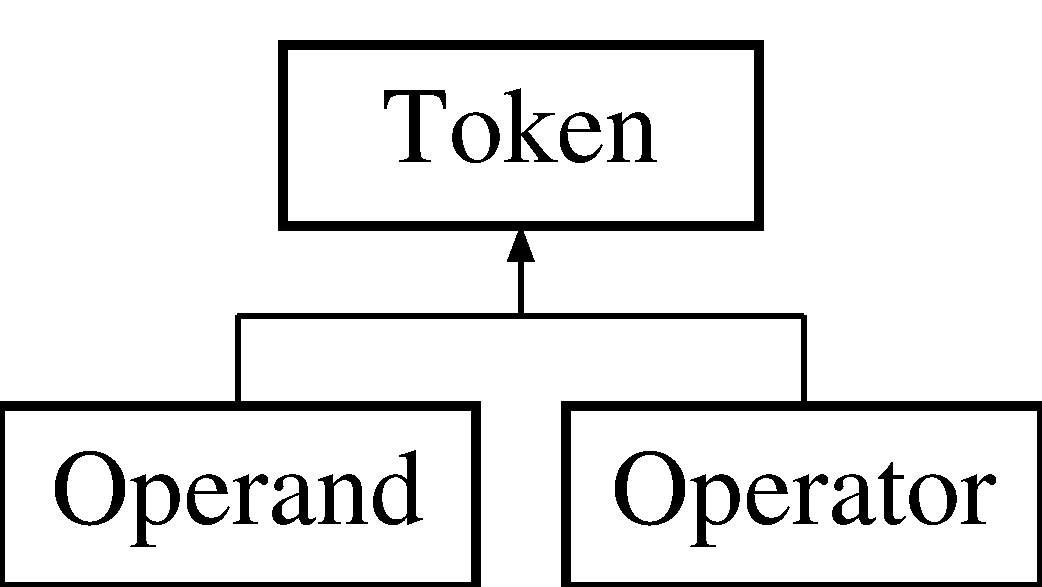
\includegraphics[height=2.000000cm]{classToken}
\end{center}
\end{figure}
\subsection*{Public Member Functions}
\begin{DoxyCompactItemize}
\item 
\hypertarget{classToken_aa1133017c00ececdf033dfb378c79e17}{{\bfseries Token} (string com, int pr=0)}\label{classToken_aa1133017c00ececdf033dfb378c79e17}

\item 
\hypertarget{classToken_acb820760827c69e98f39ca8d7ce425b0}{virtual string {\bfseries get\-Type} ()}\label{classToken_acb820760827c69e98f39ca8d7ce425b0}

\end{DoxyCompactItemize}
\subsection*{Public Attributes}
\begin{DoxyCompactItemize}
\item 
\hypertarget{classToken_a7c2cdb83b20d890bee24bdba999b0f80}{string {\bfseries command}}\label{classToken_a7c2cdb83b20d890bee24bdba999b0f80}

\item 
\hypertarget{classToken_a8125cc8499770f87f3540c81f889e039}{int {\bfseries priority}}\label{classToken_a8125cc8499770f87f3540c81f889e039}

\end{DoxyCompactItemize}
\subsection*{Protected Attributes}
\begin{DoxyCompactItemize}
\item 
\hypertarget{classToken_aa1a83620e3ce3a181768b7f8b268100c}{string {\bfseries type}}\label{classToken_aa1a83620e3ce3a181768b7f8b268100c}

\end{DoxyCompactItemize}


The documentation for this class was generated from the following file\-:\begin{DoxyCompactItemize}
\item 
token.\-h\end{DoxyCompactItemize}

\hypertarget{classTree}{\section{Tree Class Reference}
\label{classTree}\index{Tree@{Tree}}
}
\subsection*{Public Member Functions}
\begin{DoxyCompactItemize}
\item 
\hypertarget{classTree_a9537bf9697160421ba59178bf5f9d6a1}{{\bfseries Tree} (\hyperlink{classToken}{Token} t)}\label{classTree_a9537bf9697160421ba59178bf5f9d6a1}

\item 
\hypertarget{classTree_a37112c23701604aee9a580eec3b01059}{{\bfseries Tree} (\hyperlink{classToken}{Token} t, \hyperlink{classTree}{Tree} $\ast$l, \hyperlink{classTree}{Tree} $\ast$r)}\label{classTree_a37112c23701604aee9a580eec3b01059}

\end{DoxyCompactItemize}
\subsection*{Public Attributes}
\begin{DoxyCompactItemize}
\item 
\hypertarget{classTree_a462a21f3d3dfd3c257f1ec5516d4e413}{\hyperlink{classTree}{Tree} $\ast$ {\bfseries left}}\label{classTree_a462a21f3d3dfd3c257f1ec5516d4e413}

\item 
\hypertarget{classTree_a970aee4fa6894e2229a0268b224efd27}{\hyperlink{classTree}{Tree} $\ast$ {\bfseries right}}\label{classTree_a970aee4fa6894e2229a0268b224efd27}

\item 
\hypertarget{classTree_a0c9e3a9bcd2fd780b55f9562dcf4b00c}{\hyperlink{classToken}{Token} {\bfseries token}}\label{classTree_a0c9e3a9bcd2fd780b55f9562dcf4b00c}

\end{DoxyCompactItemize}


The documentation for this class was generated from the following file\-:\begin{DoxyCompactItemize}
\item 
tree.\-h\end{DoxyCompactItemize}

%--- End generated contents ---

% Index
\newpage
\phantomsection
\addcontentsline{toc}{chapter}{Index}
\printindex

\end{document}
